\chapter{Calibración}\label{appendix:calibracion}

En problemas de clasificación, el subproblema de la predicción de estimaciones
de probabilidad representativas de las probabilidades verdaderas es conocido
como calibración. En los sistemas del mundo real, los clasificadores no sólo
deben ser precisos, sino que también deben indicar cuando es probable que sean
incorrectos. Es decir, deben estimar su nivel de incertidumbre o confiabilidad.
En otras palabras, las probabilidades asociadas con la etiquetas de clase
predichas deben reflejar su verosimilitud real. Para ejemplificar este concepto
traducimos una cita de Nate Silver en su libro {\it The Signal and the Noise\/}:  

\begin{quote}
`` Una de las pruebas más importantes del pronóstico del tiempo se llama
   calibración. De todas las veces que dijiste que había un 40\% de probabilidad
   de lluvia, ¿con qué frecuencia llovió realmente? Si, a largo plazo, realmente
   llovió alrededor del 40\% de las veces, eso significa que sus pronósticos
   estaban bien calibrados. Si terminó lloviendo solo el 20\% de las veces, o el
   60\%, no fue así. ''
\end{quote}

Uno de los casos en donde se debe contemplar este problema es en la toma de
decisiones (es decir, en casi toda aplicación real). Por ejemplo, en sistemas
utilizados para la salud, un diagnóstico con un bajo nivel de confianza puede
significar realizar otro tipo de chequeo. A su vez, las estimaciones de
probabilidad, pueden ser utilizadas para ser incorporadas en otro modelo
probabilístico. Por ejemplo, se podrían combinar distintas salidas de distintos
modelos de forma ponderada para obtener una predicción más robusta frente los
casos en donde cada modelo individual falla. Sin embargo, si únicamente es de
interés la etiqueta generada por el clasificador, la calibración no aporta
valor.

Si bien la calibración parece una propiedad sencilla y quizás trivial, los
modelos mal calibrados son bastante comunes. Por ejemplo, algunos modelos están
mal calibrados desde su origen, como Naive Bayes, Random Forest y algunas redes
neuronales modernas. Incluso, hay modelos que no devuelven probabilidades {\it a
posteriori}, sino genéricas puntuaciones de confianza, como es el caso de SVM.
En estos dos últimos casos es posible mapear las salidas de los clasificadores a
probabilidades {\it a posteriori\/} calibradas a través de algunos método de
calibración~\cite{platt1999probabilistic, zadrozny2002transforming,
niculescu2005predicting, guo2017calibration}.

Dentro de los distintos modelos de clasificación, la regresión logística es un
caso especial ya que está bien calibrado por diseño, dado que su función
objetivo minimiza la función de pérdida logarítmica o {\it
log-loss\/}~\cite{morrison2013tutorial}. Sin  embargo, si no se cuenta con un
conjunto de entrenamiento lo suficientemente grande, es posible que el modelo no
tenga suficiente información para calibrar las probabilidades y sufrir la
maldición de la dimensionalidad. Las cosas se complican aún más cuando se
incorporan técnicas como regularización o {\it boosting\/}. Dadas todas las
posibles causas de una mala calibración, no se debe asumir que el modelo
ajustado estará calibrado.

Por último, una buena calibración no implica que el modelo sea bueno
clasificando. Por ejemplo, podemos tener un conjunto de datos balanceado (50\%
clase positiva, 50\% clase negativa) con el cual ajustamos un modelo que termina
clasificando aleatoriamente las observaciones en cada grupo con un 50\% de
probabilidad. Este modelo tendrá solo un 50\% de {\it accuracy\/} pero estará
calibrado de forma perfecta. Lo mismo puede ocurrir al contrario, por ejemplo,
un modelo con muy buena capacidad de clasificación pero que siempre sobrestime
las probabilidades predichas.

\section{Definición}

Matemáticamente podemos definir la calibración perfecta como:
\begin{equation}
    \mathbb{P}(\hat{Y}=y|\hat{P}=p) = p, \forall p \in [0,1]\label{ecuacion:perfect_calibration}
\end{equation}
Donde \(\hat{Y}\) es la variable aleatoria asociada a la clase predicha y
\(\hat{P}\) la de la probabilidad {\it a posteriori\/} entregada por el modelo
de clasificación. La probabilidad \(\mathbb{P}\) no puede ser computada de forma
práctica ya que \(\hat{P}\) es una variable aleatoria continua. Esto motiva la
necesidad de aproximaciones empíricas.

\section{Métodos de Calibración}

Se pueden clasificar en binarios o multiclase, y en no paramétricos y
paramétricos. Para cualquier caso, se deben conocer las $y_{i}$ clases reales
del set de calibración. Luego, para los métodos no paramétricos, debemos tener
acceso a las probabilidades $\hat p_{i}(x_i)$ estimadas por el modelo. Y para
los métodos paramétricos, debemos tener acceso a las salidas no probabilísticas
del modelo $\ z_{i}(x_i)$ o bien calcularlas haciendo $\ z_{i}(x_i) = logit(\hat
p_{i}(x_i))$ (siendo $\sigma$ la función sigmoide o logística -inversa de
$logit$-, y $\sigma_{SM}$ la función softmax, su generalización para un vector
$\boldsymbol{x}_i$).

\subsection{Modelos Binarios}

\subsubsection{Métodos no paramétricos}

\paragraph{Histograma:}

Las predicciones $\hat p_{i}(x_i)$ se dividen en {\it bins\/} $B_1, \dots B_M$
mutuamente excluyentes. Cada bin se asigna a una probabilidad calibrada
$\theta_m$ (si $\hat p_{i}(x_i)$ se asigna al bin $B_m$, entonces $\hat
q_i=\theta_m$). Al predecir, si la predicción $\hat p_t$ cae en el bin $B_m$,
entonces la probabilidad calibrada $\hat q_t$ es $\theta_m$. Los límites de los
{\it bins\/} pueden elegirse para que tengan la misma longitud o bien tengan la
misma cantidad de muestras.

\paragraph{Regresión Isotónica:}

Se estima la función por partes mediante constantes $\hat q_i=f(\hat p_i)$ que
minimiza $\sum _{i=1}^{n}(f(\hat p_{i}(x_i))-y_i)^2$. Esta técnica es una
generalización de la anterior, en la que los límites de los {\it bins\/} y las
predicciones se optimizan simultáneamente.

\paragraph{Agrupamiento bayesiano en cuantiles (BBQ):}

Es una extensión del histograma, donde mútiples opciones de {\it bins\/} son
consideradas y luego combinadas. Todas las opciones consideradas son de igual
frecuencia, pero varían en la cantidad de {\it bins\/} que emplean. Luego se
combinan mediante un score Bayesiano (que no analizaremos por su complejidad).

\subsubsection{Métodos paramétricos}

\paragraph{Platt Scaling:}

Las salidas no probabilísticas $z_{i}(x_i) = logit(\hat p_{i}(x_i))$ del
clasificador son usadas como covariables para entrenar un modelo de regresión
logística, el cual es entrenado con el set destinado a calibración para que
retorne las probabilidades reales. Es decir, la idea es estimar los parámetros
$a, b \in I\!R$ tal que $\hat q_{i} = \sigma(a.z_i+b)$. Estos parámetros se
buscan optimizando para la Negative Log-Likelihood.

\subsection{Modelos Multiclase}

\subsubsection{Métodos no paramétricos}

Una forma de extender los métodos binarios no paramétricos a multiclase es
tratando el problema como $K$ problemas de uno-vs-todos. Esto dará $K$ modelos
de calibración, cada uno para una clase en particular. Al predecir, obtenemos un
vector de probabilidades no normalizado $[\hat q_{i}^{(1)}, \dots, \hat
q_{i}^{(K)}]$ donde $\hat q_{i}^{(k)}$ es la probabilidad calibrada para la
clase $k$. Luego, esto vector es normalizado dividiendo por  $\sum
_{k=1}^{K}\hat q_{i}^{(k)}$. Esta extensión se puede aplicar a cualquiera de los
métodos no paramétricos binarios.

\subsubsection{Métodos paramétricos}

\paragraph{Vector scaling:}

Es una extensión del método de Platt Scaling, en donde se aplica una
transformación lineal $W.z_i+b$ a los $logits$:

$$\displaystyle \hat q_{i}=\max_k \sigma_{SM}(W.z_i+b)^{K}$$ Los parámetros $W$
y $b$ se buscan optimizando para la Negative Log-Likelihood. Si se restringe a
que $W$ sea diagonal, estamos dentro de la variante Vector Scaling.

\paragraph{Temparature Scaling:}

Es la extensión más simple de Platt Scaling, ya que usa un sólo parámetro $T>0$
para todas las clases. 

$$\displaystyle \hat q_{i}=\max_k \sigma_{SM}(z_i/T)^{K}$$ $T$ es llamado
temperatura, y suaviza a la función $softmax$ cuando $T>1$. A medida que
$T\to\infty$, $\hat q_{i}\to 1/K$, representando máxima incertidumbre. Con
$T=1$, se recupera la $\hat p_i$. A medida que $T \to 0$, $\hat q_{i} \to 1$. El
valor de $T$ se busca optimizando con respecto a la Negative Log-Likelihood.
Como el parámetro $T$ no altera el máximo de la función $softmax$, la predicción
de las clases post-calibración $\hat y_i '$ se mantendrán igual a las de antes
de calibrar. Es decir, que este método de calibración no cambiará el $accuracy$
del modelo.

\section{Métodos de Evaluación}

\subsection{Diagramas de confiabilidad}

También llamadas curvas de calibración, se construyen a partir de los valores
verdaderos de las clases y las probabilidades predichas para la clase principal.
Para generar una curva de calibración debemos seguir los siguientes pasos:

\begin{enumerate}
    \item Ordenar las probabilidades predichas por el modelo para la clase
    principal de menor a mayor.
    \item Dividir dichas probabilidades en $M$ bines de tamaño fijo ($1/M$).
    \item Calcular la fracción de verdaderos positivos en cada bin.
    \item Calcular el promedio de las probabilidades en cada bin.
    \item Graficar la fracción de verdaderos positivos en el eje y el promedio
    de las probabilidades en el eje x.    
\end{enumerate}

Matemáticamente, siendo $B_m$ el set de índices de las muestras cuyas
probabilidades predichas caen en el intervalo $I_m=(\frac{m-1}{M},
\frac{m}{M}]$:

\begin{equation}\label{ecuacion:acc_bm}
    acc(B_m)=\frac{1}{|B_m|}\sum _{i \in B_m}1(\hat{y_i}=y_i)
\end{equation}

donde $\hat{y_i}$ y $y_i$ son las clases predichas y reales respectivamente. Se
puede demostrar que $acc(B_m)$ es un estimador insesgado y consistente de
$P(\hat{Y}=Y|\hat{P}\in I_m)$. Por otro lado, tenemos:

\begin{equation}\label{ecuacion:conf_bm}
    conf(B_m)=\frac{1}{|B_m|}\sum _{i \in B_m}\hat{p_i}
\end{equation}

donde $\hat{p_i}$ es la probabilidad predicha para la muestra $i$.

    $acc(B_m)$ y $conf(B_m)$ aproximan el lado izquierdo y derecho
de~\ref{ecuacion:perfect_calibration} respectivamente, para el bin $B_m$. Por lo
tanto, un modelo perfectamente calibrado tendrá:

\begin{equation}\label{ecuacion:acc_conf_bm}
    acc(B_m)=conf(B_m), \forall m \in {1,\dots,M}
\end{equation}

Cuanto mejor calibrado esté el modelo, se aproximará en mayor medida la curva de
calibración obtenida a la diagonal. La curva de calibración quedará por encima
de la diagonal si el modelo tiende a subestimar las probabilidades y por debajo
si las sobreestima.

\begin{figure}[H]
    \centerline{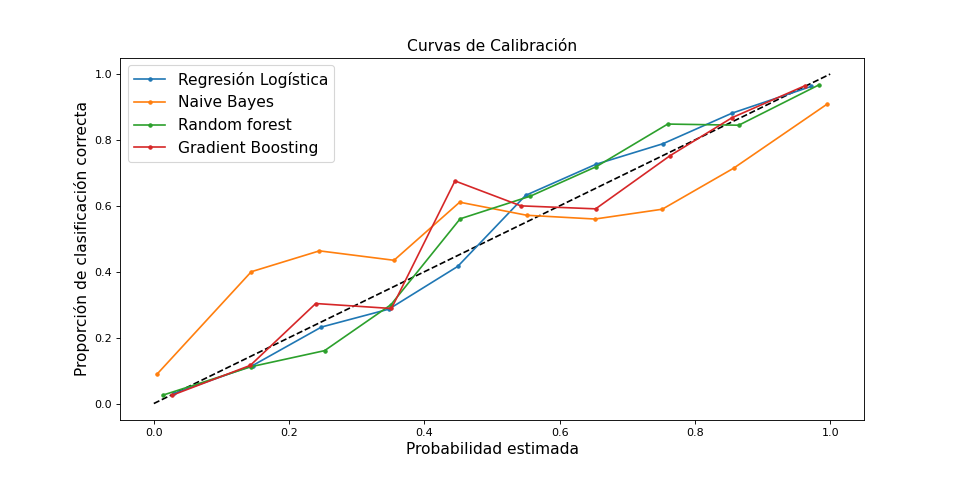
\includegraphics[width=\textwidth]{../plots_teoria/curvas_de_calibracion.png}}
    \caption{Ejemplo de curvas de calibración}\label{fig:curvas_de_calibracion}
\end{figure}

\subsection{Medidas de Evaluación}

Aunque las curvas de calibración aportan información detallada, es interesante
disponer de un único valor que permita cuantificar la calidad de calibración del
modelo. Vamos a definir primero dos medidas de evaluación que también se basan
en {\it bins\/}, y luego otras que no.

\subsubsection{Expected Calibration Error (ECE)}\label{calibracion:ECE}

Una posible medida para evaluar la descalibración podría basarse en tomar ambos
términos~\ref{ecuacion:perfect_calibration}, restarlos, y calcular el valor
esperado de la diferencia:

$$E_{\hat{P}}[|P(\hat{Y}= Y | \hat{P}=p) - p|]$$

que podemos estimar usando la siguiente fórmula:

$$ECE = \sum_{m=1}^{M} \frac{|B_m|}{n}|acc(B_m) - conf(B_m)|$$

donde $n$ es el número de muestras.

El $ECE$ es el promedio de las diferencias de los {\it bins\/} en las curvas de
calibración.

\subsubsection{Maximum Calibration Error (MCE)}\label{calibracion:MCE}

Usando el mismo concepto, pero queriendo minimizar la peor desviación, podemos
buscar:

$$\displaystyle \max_{p\in [0,1]}|P(\hat{Y}= Y | \hat{P}=p) - p|$$

el cual también se aproxima mediante {\it bins\/}:

$$\displaystyle MCE = \max_{p\in [0,1]}|acc(B_m) - conf(B_m)|$$

El $MCE$ es la máxima diferencia de los {\it bins\/} en las curvas de
calibración.

\subsubsection{Cross-Entropy}\label{calibracion:Cross-Entropy}

Teniendo en cuenta que la descalibración puede deberse a un sobreajuste de la
Cross-Entropy, podemos evaluar dicha medida en el set destinado a calibración.

$$ CE = - \frac{1}{N}\sum _{i=1}^{N} \sum _{j=1}^{M} \log \hat p_{ij}(x_i) $$
Donde $N$ es la cantidad de muestras y $M$ la cantidad de clases. Si este valor
es relativamente menor (o mayor) al del entrenamiento, es un síntoma de una
posible des-calibración. Un problema de esta medida es que da infinito si
alguna $\hat p_{ij} = 0$.

\subsubsection{Brier score}\label{calibracion:Brier score}

Otra posible medida para evaluar la bondad de ajuste de las probabilidades es el
Brier score, el cual se calcula como:

$$ BS = \frac{1}{N}\sum _{i=1}^{N} \sum _{j=1}^{M} (\hat p_{ij}(x_i) - y_{ij})^2
$$ Con respecto al Cross-Entropy, tiene la ventaja de que es siempre finito.
